\section{Trabajo Relacionado}

En esta sección se resumen los enfoques existentes que proveen soluciones
a los problemas de selección de servicios y reescritura de consultas y se
discute el trabajo relacionado en el área de inteligencia artificial llamado
compilación del conocimiento.

\subsection{Selección de Servicios}

El problema de seleccionar los servicios que implementan un flujo de trabajo
abstracto y cumplen mejor los criterios basados en QoS es conocido como el
problema de selección o composición de servicios consciente de QoS, que ha sido
demostrado ser \emph{NP-hard} \cite{Hiroshi2008}. Este es un problema de optimización
combinatoria y varias heurísticas han sido propuestas para conseguir una
solución relativamente buena en un período razonable de tiempo.

Rahmani et al. \cite{rahmani08} presentan una heurística basada en una métrica de distancia
que guía un algoritmo de búsqueda; esta métrica induce un orden de
los servicios en una manera en que los nodos vertedero (sin salida) tienen baja probabilidad
de ser visitados. En una serie de artículos, Berardi y otros \cite{berardi05,berardi08,berardi06}
describen
servicios y flujos de trabajo en términos de máquinas de estados finitos
determinísticas que son codificadas usando teorías de Lógicas Descriptivas
cuyos modelos corresponden a soluciones del problema. Aunque se podrían explotar
métodos para formalismos de Lógicas Descriptivas, no han sido reportados la
escalabilidad o el rendimiento de la solución propuesta.

Ko et al. \cite{myoung08} proponen un enfoque basado en restriccciones que codifica
los valores permisibles no funcionales como un conjunto de restricciones cuya
violación debe ser minimizada; para recorrer el espacio de soluciones
posiblemente óptima, se implementa un algoritmo híbrido que combina las
metaheurísticas \emph{tabu search} y \emph{simulated annealing}. Los resultados
experimentales muestran que la solución propuesta es capaz de escalar a un
número grande de servicios y procesos abstractos. Cardellini et al. \cite{cardellini07}
codifican una parte del problema de composición de servicios caracterizados por QoS
como un problema de programación lineal \cite{cardellini07}. Por otra parte, Wada et al.
\cite{Hiroshi2008} trata el problema como uno de optimización con múltiples objetivos donde
los diferentes parámetros de QoS son considerados igualmente importantes en vez
de ser agregados en una función. Luego se propone un algoritmo basado en
algoritmos genéticos que identifica un conjunto de composiciones de servicios
no dominadas que mejor satisfacen los requerimientos QoS.

Alrifai y Risse \cite{alrifaiR09} proponen una solución de dos fases que usa un
algoritmo de programación entera para obtener la descomposición de QoS
globales en restricciones locales y luego selecciona los servicios que mejor
cumplen las restricciones locales.

Recientemente, dos soluciones basadas en planificación han sido propuestas.
Kuter y Golbeck \cite{kuterG09} extienden el algoritmo de planificación SHOP2 para
seleccionar la composición confiable de servicios que implementan un modelo de
procesos OWL-S dado, mientras que Sohrabi y McIlraith \cite{sohrabiM09} proponen una
solución basada en planificación HTN donde las métricas de preferencia del
usario y regulaciones de dominio son utilizadas para guíar el planificador hacia
el espacio de composiciones relevantes. Finalmente, Lécué \cite{lecue09} propone un
algoritmo basado en genética para identificar la composición de servicios que
mejor cumple con los criterios de calidad para un conjunto de parámetros QoS.

Aunque estas soluciones son capaces de resolver el problema de optimización y
escalar a un número de procesos abstractos, ninguno de ellos está ajustado para
describir semánticamente los servicios en términos de procesos abstractos, ni
para usar estas descripciones para identificar los servicios que implementan un
flujo de trabajo dado o que mejor cumplen los criterios no funcionales del
usuario.

\subsection{Reescritura de Consultas}

Un número de algoritmos han sido desarrollados para encontrar las reescrituras
de una consulta dada; los más prominentes son el algoritmo \emph{bucket} \cite{levy:bucket}, el
algoritmo de reglas inversas \cite{pods:DuschkaG97,Qian96}, el algoritmo
\minicon \cite{pottinger:minicon}, y el
algoritmo \mcdsat \cite{arvelo:aaai06}. Generalmente, la reescritura de consultas trabaja en
dos fases. Durante la primera, el algoritmo identifica las vistas que reescriben
al menos un subobjetivo de la consulta, y durante el segundo estas reescrituras
parciales son combinadas en reescrituras completas. La diferencia principal
entre los algoritmos es el conjunto de criterios usado para elegir las vistas
relevantes para reducir el espacio de reescrituras no útiles.

El algoritmo denominado \emph{bucket} reduce el número de posibilidades considerando sólo cada
subobjetivo de la consulta aislado, y seleccionando las vistas que son capaces
de producir al menos los atributos proyectados por la consulta. Como los
atributos involucrados en los \emph{joins} de la consulta no son verificados, un número
grande de reescrituras comprendido por productos cartesianos puede ser generado.

El algoritmo de reglas inversas construye un conjunto de reglas que invierten
las definiciones de vistas y establecen cómo computar tuplas para las relaciones
de la base de datos a partir de las tuplas de las vistas. Al igual que el algoritmo
bucket, puede producir un gran número de reescrituras no útiles.

El algoritmo \minicon\ supera las limitaciones de los algoritmos previos
identificando solamente vistas que reescriben un conjunto de los subobjetivos de
la consulta, y que pueden ser combinados con el resto de los subobjetivos. La
idea principal es identificar las asociaciones entre variables de cada
subobjetivo a las variables en uno o más subojbetivos en las vistas, de manera
que las variables de \emph{join} de la consulta son asociadas a las variables de
\emph{join}
del cuerpo de una vista o a variables distinguidas de la vista. Asociaciones
entre variables y subojbetivos son representadas en las llamadas \emph{MiniCon
Descriptions} (MCDs) \cite{pottinger:minicon}.

Finalmente, el algoritmo \mcdsat\ es capaz de identificar las reescrituras de una
consulta traduciendo el problema de reescritura al problema de enumeración de
modelos de una teoría proposicional cuyos modelos están en correspondencia con
las reescrituras de la consulta. El algoritmo explota las propiedades de los
d-DNNF para enumerar eficientemente los modelos de la teoría.
El algoritmo
\mcdsat\ ha demostrado escalar mejor que el algoritmo \minicon\ sobre un número
grande de experimentos donde frecuentemente muestra mejoras de rendimiento de
varios órdenes de magnitud. Sin embargo, el algoritmo \mcdsat\ no fue diseñado
para problemas de reescritura que involucren constantes explícitas, ni para
computar las mejores reescrituras respecto a una función de utilidad o modelo de
costo dado. En este trabajo se propone una codificación extendida que supera
estas limitaciones y se aplica la codificación al problema de instanciación de
flujos de trabajo.

\subsection{Compilación del Conocimiento}

Compilación del conocimiento es el área en inteligencia artificial que se ocupa
del problema de traducir teorías lógicas en fragmentos apropiados que hagan
tratables ciertas operaciones deseadas \cite{cadoli:compilation}. Diferentes lenguajes de
compilación han sido definidos. Por ejemplo están los \emph{Ordered
Binary Decision Diagrams} (OBDDs) \cite{bryant:obdd},
\emph{Negation Normal Form} (NNF) \cite{barwise:handbook}, y
\emph{Decomposable Negation Normal Form} (DNNF) \cite{darwiche:map}. En este trabajo se usan las
propiedades de los DNNF determinísticos (d-DNNF) \cite{darwiche:d-dnnfs} para proveer una
solución eficiente y escalable al problema de selección de servicios.

\begin{figure}[t]
\centering
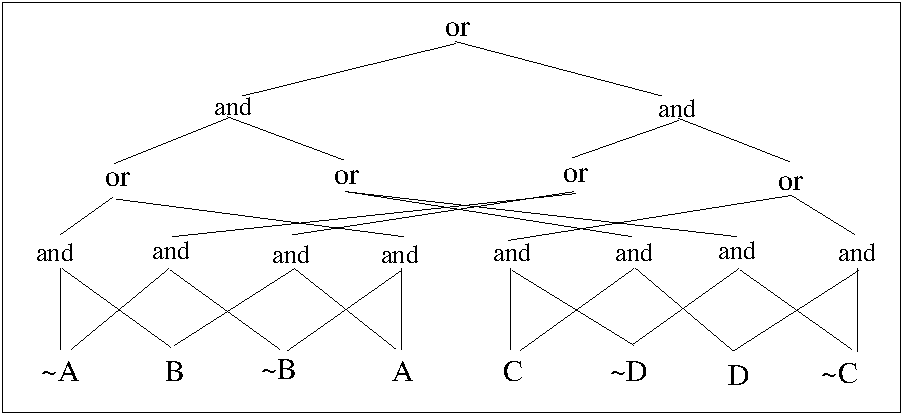
\includegraphics[width=.7\textwidth]{graphics/odd}
\caption{Un NNF descomponible y determinístico.}
\label{fig:dnnf}
\end{figure}

Una teoría en Negation Normal Form es construida desde literales usando sólo
conjunciones y disjunciones \cite{barwise:handbook}, y puede ser representada como un grafo
acíclico dirigido en que las hojas son etiquetadas con literales y los nodos
internos con $\land$ y $\lor$; ver ejemplo en la figura~\ref{fig:dnnf}. Esta
forma normal es universal, lo que significa que para cada fórmula lógica hay una
equivalente en formato NNF. Se dice que un NNF es descomponible (DNNF)
\cite{darwiche:d-dnnfs}
si para cada conjunción $\bigwedge_i\phi_i$, sus variables son disjuntas por pares; es
decir, $Vars(\phi_i)\cap Vars(\phi_j)=\empty$ para $i\neq j$. Un DNNF soporta un
número de operaciones en tiempo polinomial en el tamaño de su GAD. Por ejemplo,
podemos probar si un DNNF es satisfactible haciendo un sólo recorrido 
sobre su GAD en tiempo lineal. Se dice que un DNNF es
determinístico (d-DNNF) \cite{darwiche:d-dnnfs} si para cada disjunción $\bigvee_i\phi_i$, los
disjuntos son lógicamente contradictorios por pares, es decir,
$\phi_i\land\phi_j\equiv\textbf{false}$ para $i\neq j$.
El NNF en la figura~\ref{fig:dnnf}, por ejemplo, es
descomponible y determinístico. Un d-DNNF soporta conteo de modelos en
tiempo polinomial en el tamaño de su GAD, y enumeración de modelos en tiempo
polinomial en el tamaño de la salida. Además, dada una función de calidad de
literales $r$, se puede computar la calidad del mejor modelo en tiempo
polinomial para DNNFs \cite{darwiche:weighted}.

Toda teoría puede representarse en las formas DNNF y d-DNNF pero traducir una teoría CNF a
formato DNNF tiene costo exponencial en el peor caso. Esta traducción se
llama compilación en este campo. Hay un compilador públicamente disponible,
llamado c2d\footnote{\url{http://reasoning.cs.ucla.edu/c2d}}, que realiza este proceso de compilación y que hace uso
de técnicas de SAT modernas como backtracking dirigido por conflictos,
aprendizaje de cláusulas y caching \cite{darwiche:compiler}. Este compilador incurre en el peor
caso (peor gasto) en espacio exponencial en un parámetro llamado el ancho del árbol de
descomposición que está relacionado a la ``conectividad'' de la teoría CNF.
Sin embargo, en los experimentos realizados para esta propuesta las teorías CNF
que fueron compiladas tuvieron ancho pequeño.

